\documentclass[10pt,journal,a4paper]{IEEEtran}

% ==========================================
% MODULES ET PACKAGES DE BASE
% ==========================================
\usepackage[utf8]{inputenc}
\usepackage[T1]{fontenc}
\usepackage[french]{babel}
\usepackage{graphicx}
\graphicspath{{images/}}
\usepackage{xcolor}
\usepackage{amsmath, amsfonts, amssymb}
\usepackage{siunitx}
\sisetup{locale = FR}
\usepackage{booktabs}
\usepackage{multirow}
\usepackage{listings}

% ==========================================
% DESIGN MODERNE
% ==========================================
\definecolor{ModernBlue}{RGB}{0, 82, 155}
\definecolor{DarkGray}{RGB}{60, 60, 60}
\definecolor{CodeGray}{rgb}{0.95,0.95,0.95}

\usepackage{mathpazo} 
\usepackage[scaled]{helvet} 

\usepackage{titlesec}
\titleformat{\section}{\color{ModernBlue}\sffamily\Large\bfseries}{\thesection.}{0.5em}{}[\vspace{-0.5em}\rule{\columnwidth}{0.5pt}]
\titleformat{\subsection}{\color{ModernBlue!85}\sffamily\large\bfseries}{\thesubsection}{0.5em}{}

\usepackage{fancyhdr}
\pagestyle{fancy}
\fancyhf{} 
\renewcommand{\headrulewidth}{0.4pt} 
\renewcommand{\headrule}{\hbox to\headwidth{\color{ModernBlue}\leaders\hrule height \headrulewidth\hfill}}
\fancyhead[L]{\textcolor{DarkGray}{\sffamily RF Harvesting}}
\fancyhead[R]{\textcolor{DarkGray}{\sffamily \thepage}}
\fancyfoot[C]{\textcolor{DarkGray}{\sffamily \thepage}}

\usepackage{hyperref}
\hypersetup{colorlinks=true, linkcolor=ModernBlue, citecolor=ModernBlue, urlcolor=ModernBlue}

\lstset{
    backgroundcolor=\color{CodeGray}, 
    basicstyle=\ttfamily\small, 
    breaklines=true,
    keywordstyle=\color{ModernBlue}\bfseries, 
    commentstyle=\color{green!60!black}\itshape,
    stringstyle=\color{red}, 
    frame=single, 
    rulecolor=\color{lightgray},
    extendedchars=true,
    literate=
    {é}{{\'e}}1
    {è}{{\`e}}1
    {ê}{{\^e}}1
    {à}{{\`a}}1
    {ç}{{\c{c}}}1
    {œ}{{\oe}}1
    {ù}{{\`u}}1
    {î}{{\^i}}1
}

% ==========================================
% DÉBUT DU DOCUMENT
% ==========================================
\begin{document}

\title{\sffamily \color{ModernBlue} \Huge Rapport de Projet \\ \LARGE RF Harvesting : Récupération d'Énergie Ambiante}

\author{
    \IEEEauthorblockN{\sffamily Mathis Rudkiewicz} \\
    \IEEEauthorblockN{\sffamily Sébastien Vausort} \\
    \IEEEauthorblockA{\sffamily Option SE-ER E4a, ESEO -- 2026}
}

\maketitle
\thispagestyle{fancy} 

% --- Chargement des modules ---
\begin{abstract}
Ce document présente l'étude et la conception d'un système de récupération d'énergie par ondes radiofréquences (RF Harvesting). L'objectif est de capter l'énergie ambiante issue des réseaux Wi-Fi et cellulaires pour alimenter des capteurs IoT basse consommation, en optimisant le circuit d'adaptation d'impédance et la rectenna (antenne redresseuse).
\end{abstract}

\begin{IEEEkeywords}
RF Harvesting, Rectenna, Adaptation d'impédance, IoT, Diodes Schottky.
\end{IEEEkeywords}

\IEEEpeerreviewmaketitle
\section*{Introduction}

Energy harvesting refers to the process of capturing and converting ambient energy 
from the surrounding environment into electrical power. Among us, various 
available energy sources are existing, such as thermal, kinetic, solar, and 
radiofrequency (RF). RF energy harvesting has emerged as a particularly promising 
solution for powering autonomous, low-power electronic devices without the need for 
conventional batteries or wired power supplies.

RF energy is available almost everywhere in the electromagnetic spectrum through 
everyday wireless technologies such as Wi-Fi routers, cellular base stations, 
television broadcast towers, and Bluetooth devices. Although the power density of 
these ambient RF signals is relatively low, recent advances in rectenna (rectifying 
antenna) design and ultra-low-power electronics have made it feasible to harvest 
sufficient energy for more and more applications, including wireless sensor networks, 
implantable medical devices, and Internet of Things (IoT) sensors.

A rectenna is the core component of any RF energy harvesting system. It consists of 
a receiving antenna coupled to a rectifying circuit, which converts the incoming 
alternating current (AC) RF signal into a usable direct current (DC) voltage. As 
illustrated in Figure~\ref{fig:rf_system}, a complete RF energy harvesting chain 
typically includes a matching circuit, a voltage multiplier (rectifier), an energy 
storage element, and a microcontroller unit driving the target application. The 
overall performance of such a system is primarily characterized by its RF-to-DC 
power conversion efficiency (PCE), defined as:

\begin{equation}
    \eta_{RF-DC} = \frac{P_{DC}}{P_{RF}} = \frac{V_{DC}^2 / R_L}{P_{RF}}
\end{equation}

\noindent where $P_{RF}$ is the available input RF power, $V_{DC}$ is the output DC 
voltage, and $R_L$ is the load resistance. Maximizing this efficiency requires 
careful co-design of the antenna, the impedance matching network, and the rectifier 
topology.

\begin{figure}[h]
    \centering
    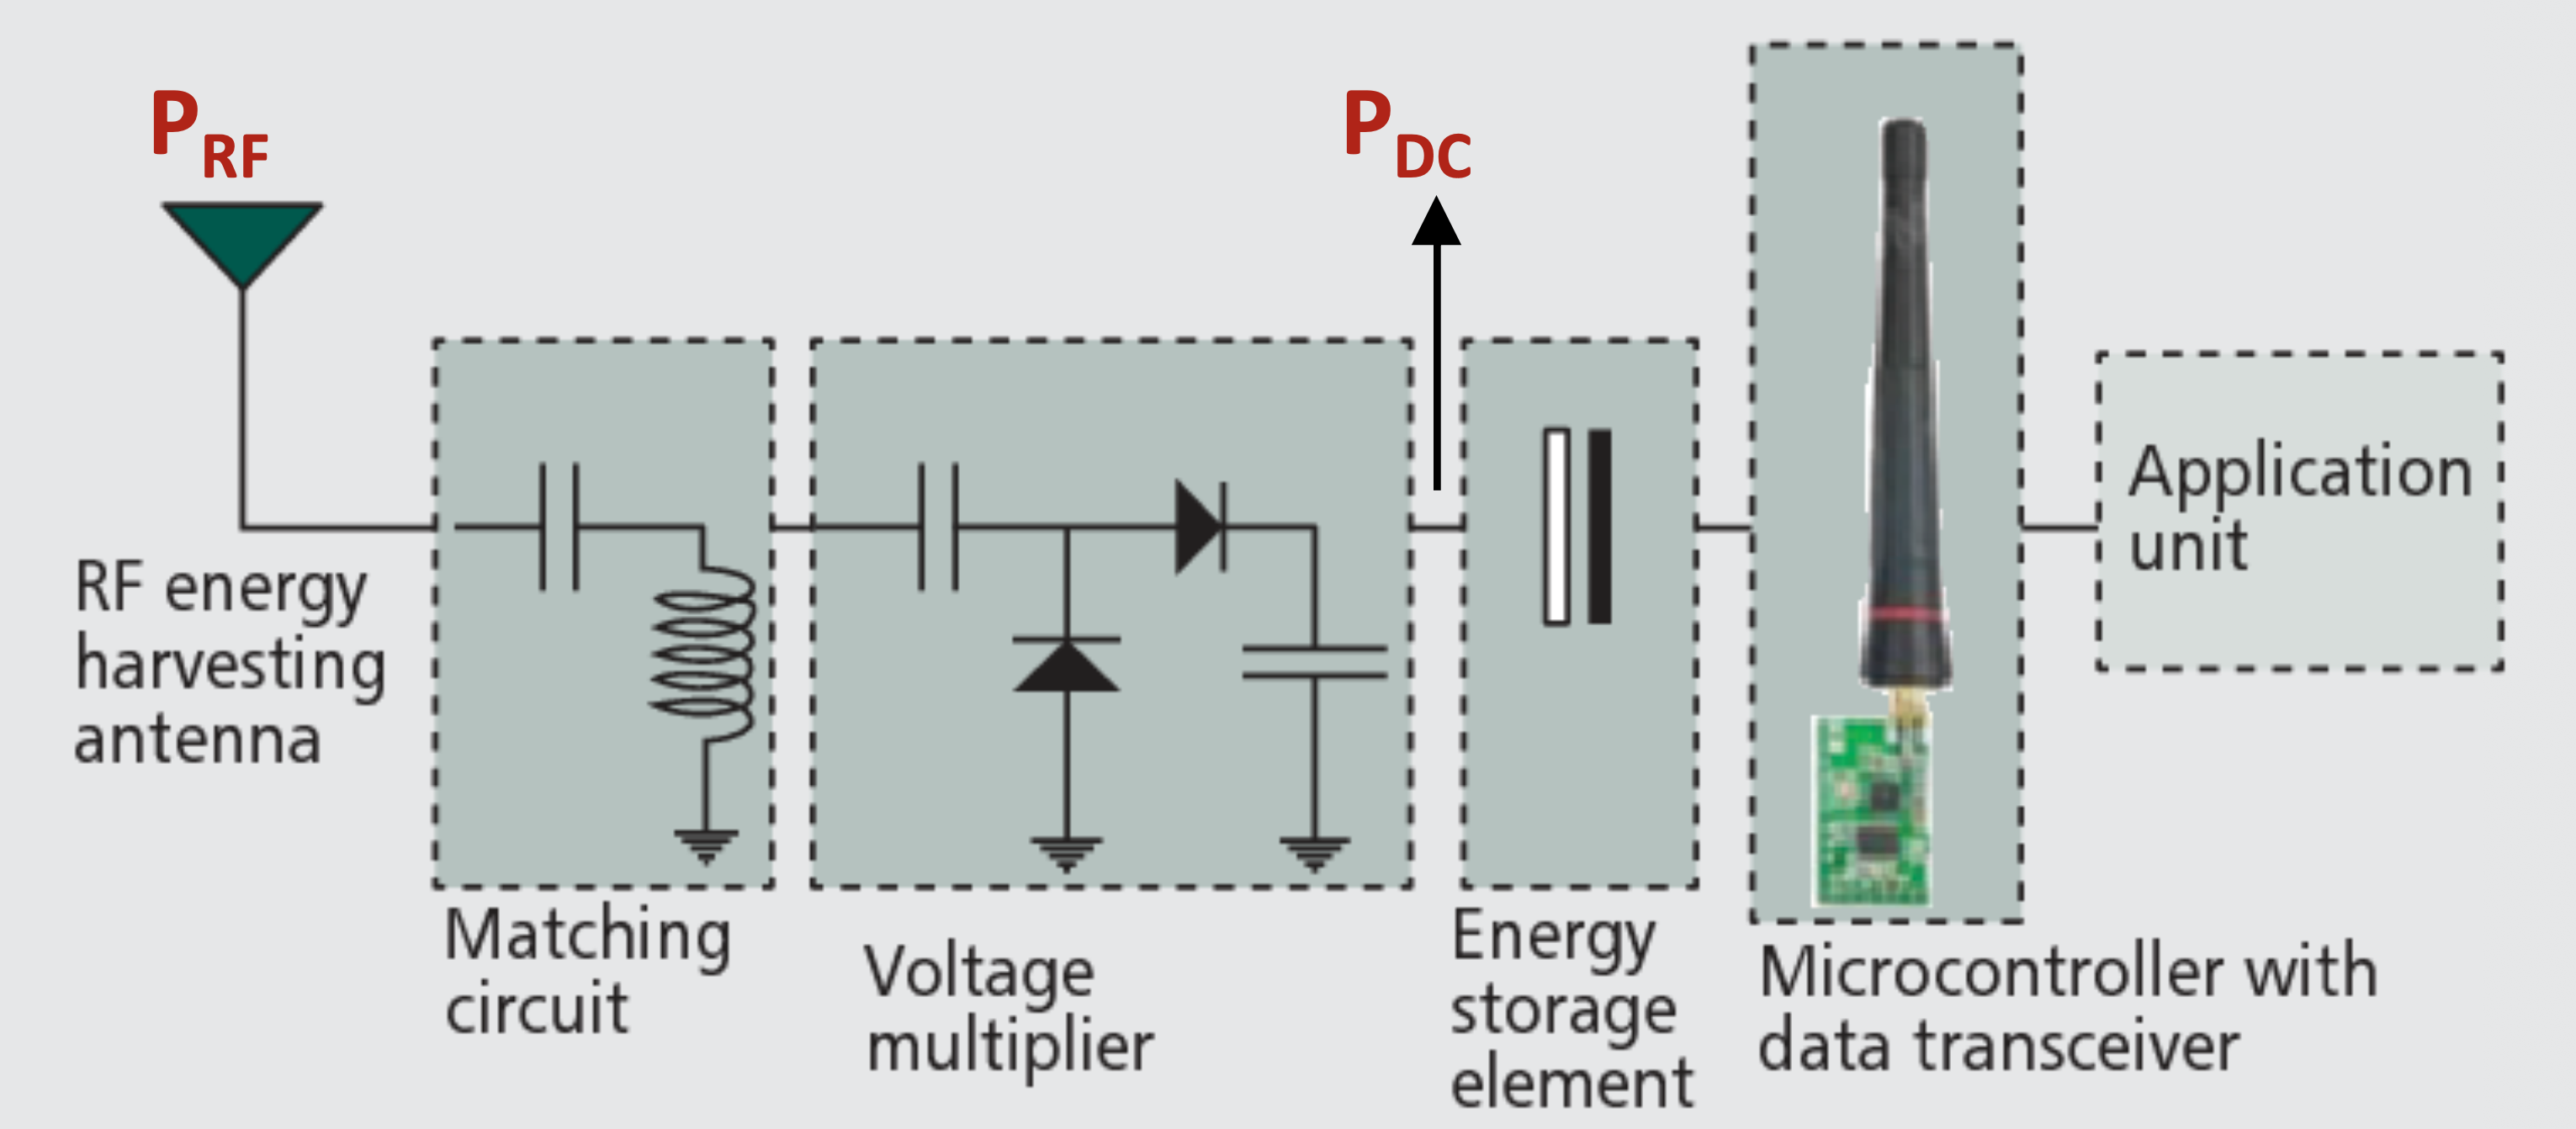
\includegraphics[width=0.45\textwidth]{systeme_rf.png}
    \caption{Block diagram of a complete RF energy harvesting system, from the 
    receiving antenna ($P_{RF}$) to the application unit ($P_{DC}$).}
    \label{fig:rf_system}
\end{figure}

The rectifier topology plays a critical role in determining both the conversion 
efficiency and the output voltage level. Figure~\ref{fig:topologies} presents the 
three conventional rectenna topologies considered in the literature: the series 
topology (a), the shunt topology (b), and the single voltage doubler topology (c). 
In this study, the one-diode (series or shunt) and the two-diode (voltage doubler) 
configurations are designed, simulated, and experimentally compared.

\begin{figure}[h]
    \centering
    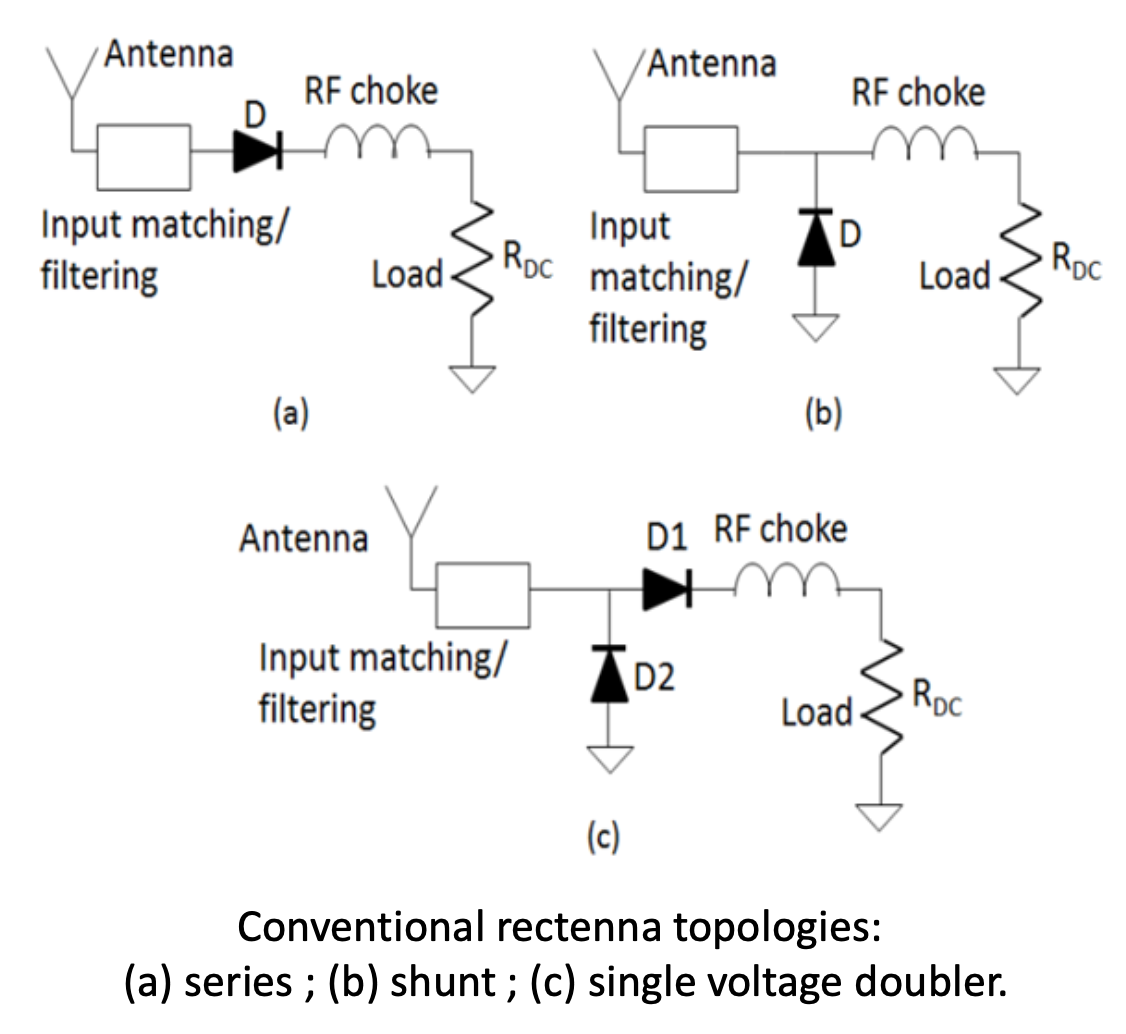
\includegraphics[width=0.45\textwidth]{topologies.png}
    \caption{Conventional rectenna topologies: (a) series; (b) shunt; 
    (c) single voltage doubler.}
    \label{fig:topologies}
\end{figure}

The objective of this practical work is to design, simulate, and characterize two AC to DC converter topologies, a one-diode topology and a 
two-diode topology, for low-power RF energy harvesting. Analysis are 
carried out using the Keysight Advanced Design System (ADS) professional software, 
with operating frequencies selected within the 1.5--3~GHz range, covering widely 
used ISM bands such as 2.45~GHz. Both lumped-element (LC) and distributed impedance (microstrip line) matching strategies are investigated and compared.

The report is structured as follows. Section~\ref{sec:task2} presents the choice 
of application, operating frequency, and Schottky diode. Section~\ref{sec:task3} 
details the design and simulation of the one-diode rectifier topology, including 
impedance matching optimization. Section~\ref{sec:task4} extends this analysis to 
the two-diode configuration. Section~\ref{sec:task5} describes the PCB design, 
fabrication process, and experimental measurements. Finally, a comparative 
discussion and conclusion are provided, assessing the suitability of each topology 
for the targeted low-power application.
\section{Task 1 : Impedance Matching}
\label{sec:task1}

\subsection{Goals of this task}
The main objective of this step is to design a matching circuit to maximize energy transfert from
 an input impedance of an antenna and an output impedance of a Schottky diode. 
 In an RF harvesting system, an antenna circuit have an impedance ($Z_{in}$) of 50 $\Omega$. 
 This is a compromise between loss and power transmission. On the other hand, a Schottky diode 
 (who act like a charge) have a complex impédance ($Z_{diode}$) which is not fix regarding the frequency 
 of the system. Without any adaptation, there will be a high reflexion of catched energy by the antenna, 
 this problem will minimize the efficiency of our system.

\subsection{Modelling}

To simulate the behavior with the Keysight ADS software, we wanted to transform the complexe impédence 
of the diode to passives components like resistors, capacitors and inductors. There is the complex form of an impedance :  

\begin{equation} \label{eq:complex_form_impedance}
    Z = R + jX
\end{equation}

The real part ($R$) represent the resistive part of the diode. 
This is why this part is modelized by a simple resistor in the simulator.

The imaginary part ($X$) is the reactance of the component. 
With a Schottky diode, this reactance is negative, that means that we can replace this with a capacitor in the software

To modelize this imaginary part in the simulator, we need to calculate the capacitor’s value. 
We used this equation de determine this value

\begin{equation} \label{eq:capacitor_value}
    C = -\frac{1}{2\pi f X}
\end{equation}

\subsection{Expected results}

When the diode was modelized by its equivalent RC circuit, we added a LC filter between the source (50 $\Omega$) 
and the charge (Schottky diode). This filter’s objective is to compensate the imaginary part of the diode and 
keep a 5O $\Omega$ impedance at the expected frequency.

We use a method included in the Keysight’s software. This is a tool to tune dynamicaly the value of the 
inductance and the capacitor of the filter. The goal is to find a “dip” in the chart at the expected frequency. 
this “dip” is the optimal resonance of the system. Regarding the specifications, we want to obtain a $S_{11}$ 
parameter (reflexion coeficient) lower than -10 db at the wanted frequency.
\section{Task 2 : Choice of application, diode and frequency}
\label{sec:task2}

\subsection{Sensor and frequency}
For the project, we needed to supply an ultra low power sensor. The choosed component is STTS22H, 
a temperature sensor made by STMicroelectronics. We can justify this choice with its ideals caracteristics 
for energy harvesting. It’s an I2C temperature sensor working between 1.5V and 3.6V and it can be on with 
an ultra low supply current under 120 µA. To harvest ambient energy, we choosed 2.2 GHz frequency. 
This frequency is between 1.5 and 3 GHz wanted in the specifications.

\subsection{CMOS Diodes vs Schottky Diodes}
Harvesting RF signals (which are often very weak, around a microwatt) requires an extremely sensitive and fast AC-DC rectifier.

- CMOS Diodes (P-N Junction): These are based on a junction of P-doped and N-doped semiconductors. 
They have a relatively high threshold voltage (usually between 0.6 V and 0.7 V). 
Additionally, their switching time is limited by the recombination of minority charge carriers. 
Therefore, they are not suitable for rectifying very weak, high-frequency RF signals.

- Schottky Diodes: These use a metal-semiconductor junction. This structure provides a much lower threshold voltage 
(typically between 0.15 V and 0.3 V), allowing the rectification to start even with very low input power. 
Moreover, since the current is carried by majority carriers, there is no delay caused by recombination. 
This enables the ultra-fast switching required at gigahertz (GHz) frequencies.

\subsection{BAV99 and HSMS-28xx series diodes}
The BAV99 is a standard silicon switching diode (P-N). Because of its high threshold voltage 
and large junction capacitance, it would severely weaken the signal at 2.2 GHz. It would also 
require much more input power than an energy harvesting antenna can actually provide.

The HSMS-28xx series consists of Schottky diodes specifically designed for RF detection and energy harvesting. 
They are optimized to offer minimal junction capacitance (Cj) and very low series resistance (Rs), 
which maximizes the RF-to-DC conversion efficiency.

\subsection{Which diode do we need ?}

We compared three models from the HSMS series to find the best diode for our 2.2 GHz target frequency. 
The HSMS-2850 has a low threshold voltage, but it is designed to operate at frequencies below 1.5 GHz. 
Therefore, we cannot use it for our 2.2 GHz application. The HSMS-2820 can work up to 4 GHz, but it has a 
junction capacitance of 0.7 pF. At 2.2 GHz, this capacitance would cause significant insertion losses. 
The HSMS-2860 works up to 5.8 GHz and has a very low junction capacitance of 0.18 pF.

The HSMS-2860 diode is the best choice for our matching and rectifying circuit at 2.2 GHz. 
Its low parasitic parameters will guarantee the best conversion efficiency to power the STTS22H sensor.

\begin{table}[h]
    \centering
    \caption{Schottky diodes compraison for RF energy harvesting applications at 2.2 GHz.}
    \label{tab:diodes_comparison}
    \begin{tabular}{lcccc}
        \toprule
        \textbf{Diode} & \textbf{($I_s$)} & \textbf{($R_s$)} & \textbf{($C_j$)} & \textbf{($F$)}\\
        \midrule
        HSMS-2820 & \SI{22}{\nano\ampere} & \SI{6}{\ohm} & \SI{0.7}{\pico\farad} & up to \SI{4}{\giga\hertz} \\
         HSMS-2850 & \SI{3000}{\nano\ampere} & \SI{25}{\ohm} & \SI{0.18}{\pico\farad} & below \SI{1.5}{\giga\hertz} \\
        HSMS-2860   & \SI{50}{\nano\ampere} & \SI{6}{\ohm} & \SI{0.18}{\pico\farad} & up to \SI{5.8}{\giga\hertz} \\
        \bottomrule
    \end{tabular}
\end{table}
% ============================================================
%  TASK 3.1 — ONE-DIODE RECTIFIER TOPOLOGY
%  RF Harvesting Report — Rudkiewicz & Vausort — ESEO 2026
% ============================================================
% Required packages (add to your main preamble if not present):
%   \usepackage{amsmath, amssymb}
%   \usepackage{booktabs}
%   \usepackage{graphicx}
%   \usepackage{siunitx}
%   \usepackage{hyperref}
%   \usepackage{caption}
%   \usepackage{subcaption}
%   \usepackage{float}          % <-- required for [H] float specifier
%
% Also add this in your preamble after \usepackage{siunitx}:
%   \DeclareSIUnit{\dBm}{dBm}
% ============================================================

% ----- If this file is \input directly, uncomment the two lines below -----
% \usepackage{float}
% \DeclareSIUnit{\dBm}{dBm}

\section{Task 3.1 --- One-Diode Rectifier Topology}
\label{sec:task3_1}

This part presents the full characterization of the one-diode rectifier
topology implemented with the HSMS-2860 Schottky diode at an operating
frequency of \SI{2.2}{\giga\hertz}.
The analysis will follow a systematic progression : (1) characterization of the diode
input impedance without any matching network, (2) study of its dependence on
input power and load resistance, (3) design and validation of the lumped-element
impedance matching circuit, (4) extension to a microstrip implementation
including design rule constraints, and (5) evaluation of the one-diode rectifier topology
performance in terms of conversion efficiency~$\eta$, output voltage~$V_\mathrm{out}$,
and output current~$I_\mathrm{out}$.
% ------------------------------------------------------------
\subsection{Diode Input Impedance vs.\ Frequency (without Matching Circuit)}
\label{subsec:zin_vs_freq}
% ------------------------------------------------------------


Before extracting the diode input impedance, it is important to understand the
structure of the one-diode rectifier simulated in ADS, shown in
Figure~\ref{fig:schematic_one_diode}.
The circuit is composed of the following elements:

\begin{itemize}
    \item \textbf{RF source:} a single-tone power source \texttt{P\_1Tone}
          (PORT1, $Z = \SI{50}{\ohm}$) sweeping from \SIrange{1}{3}{\giga\hertz},
          delivering a power $P = \mathrm{polar}(\mathrm{dbmtow}(P_\mathrm{in}), 0)$,
          which converts the input power from dBm to Watts in polar form. It simulates the antenna behavior. 

    \item \textbf{DC-blocking / RF choke network:} two capacitors
      $C_1 = C_2 = \SI{100}{\pico\farad}$ placed in series on the 
      signal path and in shunt at the output respectively.
      $C_1$ blocks any DC component from reaching the source, while 
      $C_2$ shorts the RF signal to ground at the output node, acting 
      as an RF bypass capacitor that forces the load to see only the 
      rectified DC voltage.

    \item \textbf{Schottky diode D1:} the HSMS-2860 model is placed in series between the
          RF input and the output node.
          In this series topology, the diode rectifies the RF signal by conducting
          only during positive half-cycles, charging $C_2$ to a DC voltage.

    \item \textbf{Load resistor:} $R_1 = R_L$, represents the equivalent
          input resistance of tour sensor (STTS22H).
          Here we have, $R_L = \SI{10}{\kilo\ohm}$ for the moment.
\end{itemize}

More on the simulation and measurements parts, we have two current probes (\texttt{I\_Probe1} on the input path, \texttt{I\_Probe2}
on the output path). They are respectively measuring the RF input current and the DC output current. On the other side, 
the LSSP harmonic-balance solver is a linear $S$-parameter
simulation because the diode is a nonlinear component (its behavior
depends on the RF level, this force us large to use signal analysis). Finaly, the impedance $Z_\mathrm{in}$ is extracted via the ADS equation block:
\texttt{Zin1 = zin(S11, PortZ1)}.

\begin{figure}[htbp]
    \centering
    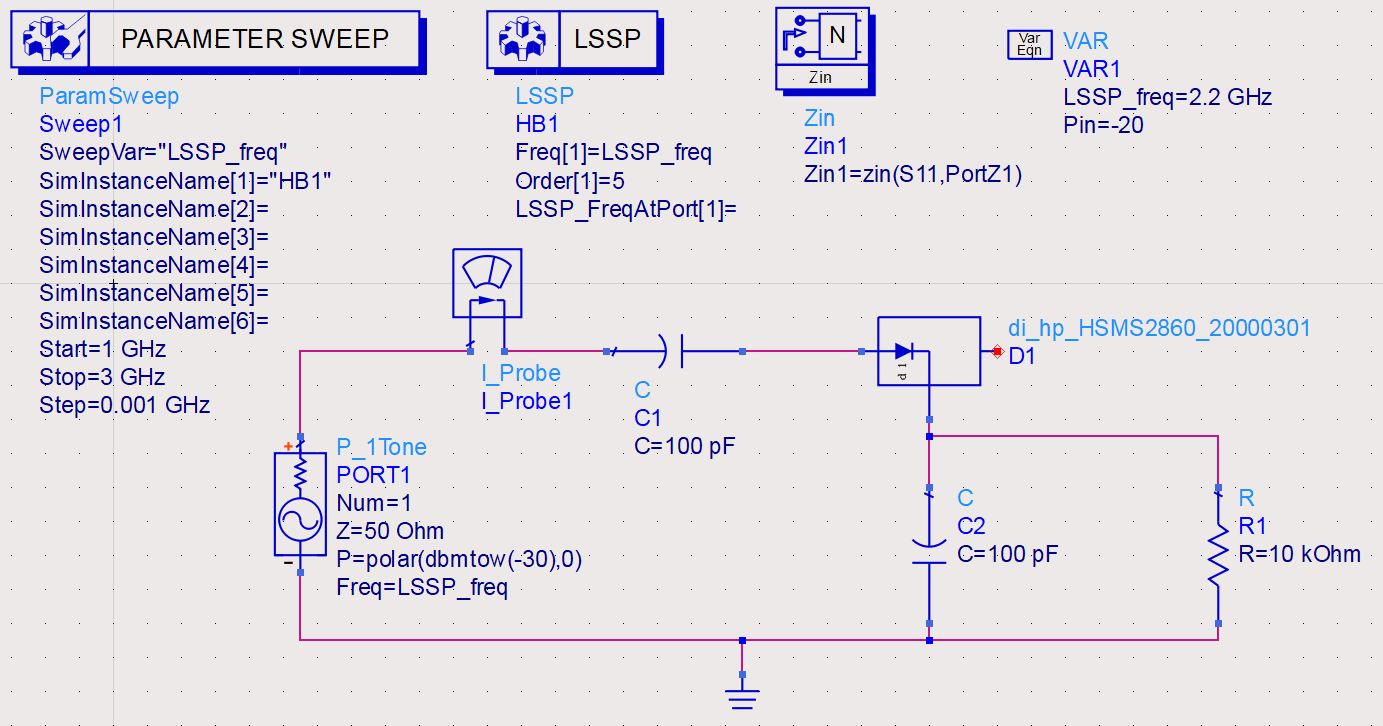
\includegraphics[width=\linewidth]{images/schematic_one_diode.png}
    \caption{ADS schematic of the one-diode series rectifier used for
             input impedance extraction.}
    \label{fig:schematic_one_diode}
\end{figure}

\subsubsection{Simulation setup}

The input impedance $Z_\mathrm{indiode}$ of the HSMS-2860 is extracted using
a LSSP (Large-Signal S-Parameter) simulation in Keysight ADS over the
frequency range \SIrange{1}{3}{\giga\hertz}, with a frequency step of
\SI{1}{\mega\hertz}.
The operating conditions are fixed at $P_\mathrm{in} = -20\,\text{dBm}$ and
$R_L = \SI{10}{\kilo\ohm}$.
The problem is that, the input impedance $Z_\mathrm{in}$ of the diode cannot be measured 
directly in ADS. Instead, the simulator measures the reflection 
coefficient $S_{11}$ at Port~1, which represents the ratio of the 
reflected wave to the incident wave at the port. Since any impedance 
mismatch between the source ($Z_0 = \SI{50}{\ohm}$) and the diode 
causes a partial reflection of the incident signal, $S_{11}$ has 
the full information needed to recover $Z_\mathrm{in}$. The conversion could be done by using this relation:
%
\begin{equation}
    Z_\mathrm{in} = Z_0 \,\frac{1 + S_{11}}{1 - S_{11}},
    \label{eq:zin_from_s11}
\end{equation}
%
which is evaluated in ADS via the built-in function 
\texttt{zin(S11, PortZ1)}.
If $S_{11} = 0$ (no reflection), 
and gives $Z_\mathrm{in} = Z_0 = 
\SI{50}{\ohm}$, confirming perfect matching. On the other hand, if $S_{11} = -1$ 
(total reflection, short circuit), it gives $Z_\mathrm{in} = 0$.

Regarding the two \SI{100}{\pico\farad} capacitors $C_1$ and $C_2$: 
at \SI{2.2}{\giga\hertz}, their impedance is only
$X_C = 1/(2\pi f C) \approx \SI{0.72}{\ohm}$, which is negligible 
compared to $Z_0 = \SI{50}{\ohm}$. Therefore the behave as 
short-circuits at RF frequencies and do not disturb the impedance 
measurement of the diode. At DC, a capacitor blocks any 
current flow, this means that $C_1$ prevents the 
rectified DC voltage from flowing back into the source, and $C_2$ 
ensures that the load $R_L$ receives a clean DC voltage.

% ------------------------------------------------------------
\subsection{Influence of \texorpdfstring{$P_\mathrm{in}$}{Pin} and
            \texorpdfstring{$R_L$}{RL} on \texorpdfstring{$Z_\mathrm{in,diode}$}{Zin}}
\label{subsec:zin_tables}
% ------------------------------------------------------------

\subsubsection{Effect of input power at fixed \texorpdfstring{$R_L = \SI{10}{\kilo\ohm}$}{RL=10kohm}}

The LSSP simulation is repeated for five input power levels
($P_\mathrm{in} \in \{-30, -20, -10, 0, +10\}$\,dBm) with $R_L = \SI{10}{\kilo\ohm}$
fixed.
Table~\ref{tab:zin_vs_pin} summarizes the extracted impedance values at
\SI{2.2}{\giga\hertz}.

\begin{table}[htbp]
    \centering
    \caption{Real and imaginary parts of $Z_\mathrm{in,diode}$ at \SI{2.2}{\giga\hertz}
             for varying $P_\mathrm{in}$, with $R_L = \SI{10}{\kilo\ohm}$.}
    \label{tab:zin_vs_pin}
    \begin{tabular}{S[table-format=-2.0]
                    S[table-format=1.3]
                    S[table-format=-3.3]}
        \toprule
        {$P_\mathrm{in}$ (dBm)} &
        {$\mathrm{Re}(Z_\mathrm{in})$ ($\Omega$)} &
        {$\mathrm{Im}(Z_\mathrm{in})$ ($\Omega$)} \\
        \midrule
        -30 & 2.580 & -259.618 \\
        -20 & 2.533 & -263.520 \\
        -10 & 2.517 & -279.632 \\
          0 & 2.781 & -320.298 \\
         10 & 3.282 & -393.890 \\
        \bottomrule
    \end{tabular}
\end{table}

\paragraph{Analysis.}
Two distinct trends emerge from Table~\ref{tab:zin_vs_pin}:
%
\begin{itemize}
    \item \textbf{Real part:} $\mathrm{Re}(Z_\mathrm{in})$ remains quasi-constant
    across the full power range, varying only from \SI{2.517}{\ohm} to
    \SI{3.282}{\ohm}.
    This is consistent with the physics of the HSMS-2860: the series resistance
    $R_s$ is a bulk property of the metal-semiconductor junction, largely
    independent of the signal level over this range.

    \item \textbf{Imaginary part:} $\mathrm{Im}(Z_\mathrm{in})$ becomes
    increasingly negative as $P_\mathrm{in}$ rises.
    At $P_\mathrm{in} = +10\,\text{dBm}$, the reactance reaches
    $\SI{-393.89}{\ohm}$, compared to $\SI{-259.62}{\ohm}$ at
    $P_\mathrm{in} = -30\,\text{dBm}$.
    This behavior reflects the voltage-dependent nature of the Schottky
    junction capacitance: as the RF voltage swing increases, the average
    junction bias shifts, changing the effective capacitance $C_j(V)$.
\end{itemize}
%
This power-dependency implies that the impedance matching circuit designed for
a specific power level may perform sub-optimally at other power levels.
In a practical low-power RF harvesting scenario ($P_\mathrm{in} \leq -20\,\text{dBm}$),
the variation is small enough to be neglected for a first-order design.

\subsubsection{Effect of load resistance at fixed \texorpdfstring{$P_\mathrm{in} = -20\,\text{dBm}$}{Pin=-20dBm}}

Table~\ref{tab:zin_vs_rl} presents the impedance values for three different
load resistances ($R_L \in \{1, 5, 10\}$\,k$\Omega$) at
$P_\mathrm{in} = -20\,\text{dBm}$.

\begin{table}[htbp]
    \centering
    \caption{Real and imaginary parts of $Z_\mathrm{in,diode}$ at \SI{2.2}{\giga\hertz}
             for varying $R_L$, with $P_\mathrm{in} = -20\,\text{dBm}$.}
    \label{tab:zin_vs_rl}
    \begin{tabular}{S[table-format=2.0]
                    S[table-format=1.3]
                    S[table-format=-3.3]}
        \toprule
        {$R_L$ (k$\Omega$)} &
        {$\mathrm{Re}(Z_\mathrm{in})$ ($\Omega$)} &
        {$\mathrm{Im}(Z_\mathrm{in})$ ($\Omega$)} \\
        \midrule
         1 & 2.522 & -263.520 \\
         5 & 2.522 & -263.520 \\
        10 & 2.522 & -263.520 \\
        \bottomrule
    \end{tabular}
\end{table}

\paragraph{Analysis.}
The impedance is completely insensitive to the load resistance over the range
tested: both $\mathrm{Re}(Z_\mathrm{in})$ and $\mathrm{Im}(Z_\mathrm{in})$
remain strictly constant at \SI{2.522}{\ohm} and \SI{-263.520}{\ohm}
respectively.
This result is physically expected: at RF frequencies (\SI{2.2}{\giga\hertz}),
the LSSP simulation captures the small-signal RF behavior of the diode at its
operating point.
The load resistance $R_L$ only influences the DC bias point of the rectifier
through the output DC voltage, but its effect on the high-frequency
small-signal junction impedance is negligible when $R_L \gg 1/(\omega C_j)$.
Indeed, $1/(\omega C_j) \approx 1/(2\pi \times 2.2 \times 10^9 \times
0.18 \times 10^{-12}) \approx \SI{402}{\ohm}$, which is far smaller than
any of the tested load values.

The key practical implication is that the impedance matching network can be
designed independently of the load resistance for the targeted application
(STTS22H sensor, $R_L \approx \SI{10}{\kilo\ohm}$), which simplifies the
design process considerably.

% ------------------------------------------------------------
\subsection{Lumped-Element Impedance Matching Circuit}
\label{subsec:matching_lumped}
% ------------------------------------------------------------

\subsubsection{Design methodology}

The objective of the matching network is to transform the antenna source
impedance $Z_0 = \SI{50}{\ohm}$ to the complex conjugate of the diode input
impedance $Z_\mathrm{in,diode}^*$, so as to maximize power transfer.
The design employs the ADS dynamic tuning tool (\emph{Tune}) to iteratively
adjust the component values while observing $S_{11}$ and $Z_\mathrm{in}$
in real time.
The target specification is:
%
\begin{equation}
    S_{11}(f = \SI{2.2}{\giga\hertz}) < \SI{-10}{\deci\bel}.
    \label{eq:s11_spec}
\end{equation}

The matching topology selected is a two-stage LC ladder network inserted
between the RF port and the diode.
This topology uses the following real SMD components:
%
\begin{itemize}
    \item Two shunt capacitors: $C_7 = \SI{3.3}{\pico\farad}$ and
          $C_8 = \SI{3.9}{\pico\farad}$ (series UPY-AQ NP0, 16--50\,V);
    \item Two series inductors: $L_2 = \SI{18}{\nano\henry}$ and
          $L_3 = \SI{8.2}{\nano\henry}$.
\end{itemize}
%
All components are modeled in ADS using their $\mathrm{C\_Pad1}$ and
$\mathrm{L\_Pad1}$ footprint models (0603 SMD package), which include the
parasitic elements associated with the physical pad geometry:
$W = \SI{0.8}{\milli\meter}$, $S = \SI{0.4}{\milli\meter}$,
$L_1 = \SI{1.6}{\milli\meter}$ for the capacitors, and
$W = \SI{0.64}{\milli\meter}$, $S = \SI{0.56}{\milli\meter}$,
$L_1 = \SI{1.19}{\milli\meter}$ for the inductors.

\subsubsection{Results after tuning}

After optimization, the resulting impedance at \SI{2.2}{\giga\hertz} is:
%
\begin{align}
    \mathrm{Re}(Z_\mathrm{in})\big|_\mathrm{matched}
        &= \SI{48.652}{\ohm}, \\
    \mathrm{Im}(Z_\mathrm{in})\big|_\mathrm{matched}
        &= \SI{-10.990}{\ohm}.
\end{align}
%
The optimal tuning values found by the ADS Tune tool are
$\mathrm{Cap} = \SI{7.286}{\pico\farad}$ and
$\mathrm{Ind} = \SI{26.247}{\nano\henry}$, which guided the selection of
the nearest standard commercial values ($C_7 = \SI{3.3}{\pico\farad}$,
$C_8 = \SI{3.9}{\pico\farad}$, $L_2 = \SI{18}{\nano\henry}$,
$L_3 = \SI{8.2}{\nano\henry}$).

The $S_{11}$ parameter of the matched circuit reaches
\textbf{\SI{-21.84}{\deci\bel}} at \SI{2.2}{\giga\hertz}, as shown in
Figure~\ref{fig:s11_matched_lumped}, which satisfies the specification
of~(\ref{eq:s11_spec}) with a margin of more than \SI{11}{\deci\bel}.

\begin{figure}[htbp]
    \centering
    % \includegraphics[width=0.75\linewidth]{figures/s11_matched_lumped.png}
    \caption{$S_{11}$ parameter of the one-diode rectifier with the
             lumped-element matching circuit ($C_7 = 3.3$\,pF,
             $C_8 = 3.9$\,pF, $L_2 = 18$\,nH, $L_3 = 8.2$\,nH).
             $R_L = 10$\,k$\Omega$, $P_\mathrm{in} = -20$\,dBm.
             Marker m3: $S_{11}(2.2\,\mathrm{GHz}) = -21.84$\,dB.}
    \label{fig:s11_matched_lumped}
\end{figure}

\subsubsection{Asymmetry of the \texorpdfstring{$S_{11}$}{S11} response}

A notable feature of the $S_{11}$ curve in Figure~\ref{fig:s11_matched_lumped}
is its pronounced \emph{asymmetry} around the resonance frequency.
The response rises steeply on the low-frequency side and rolls off more
gradually on the high-frequency side, rather than presenting a symmetric
band-pass shape.

This asymmetry is a direct consequence of using a \textbf{single diode}
topology.
The Schottky diode acts as a nonlinear, non-reciprocal element: it conducts
preferentially during positive half-cycles of the RF signal, creating a
half-wave rectification process.
This introduces even-order harmonic distortion and a DC offset that modulates
the effective junction impedance differently on each side of resonance.
In a two-diode topology (voltage doubler), the two diodes conduct on opposite
half-cycles, and their nonlinear contributions cancel to first order, restoring
a more symmetric $S_{11}$ profile.
This difference will be examined further in the comparative analysis of
Section~\ref{sec:task4}.

% ------------------------------------------------------------
\subsection{Extension to Microstrip Implementation}
\label{subsec:matching_microstrip}
% ------------------------------------------------------------

\subsubsection{Substrate and design rules}

The physical PCB implementation follows the design rules specified for this
project:
%
\begin{itemize}
    \item Substrate: Rogers 4350B ($\varepsilon_r = 4.5$,
          $\tan\delta = 0.02$, $H = \SI{1.6}{\milli\meter}$,
          copper thickness $T = \SI{0}{\milli\meter}$ in ADS model);
    \item Signal traces: characteristic impedance $Z_0 = \SI{50}{\ohm}$,
          corresponding to $W = \SI{3.034}{\milli\meter}$;
    \item Microstrip line length constraints:
          $\SI{3}{\milli\meter} \leq L_\mathrm{line} \leq \SI{10}{\milli\meter}$;
    \item SMD package: 0603.
\end{itemize}
%
Each lumped component (capacitor, inductor) is surrounded by two MLIN
microstrip segments on either side, connected through MTEE-ADS T-junction
elements to model the physical routing on the PCB.
All line segments use $W = \SI{3.034}{\milli\meter}$, consistent with
$Z_0 = \SI{50}{\ohm}$.

\subsubsection{Effect of microstrip parasitics on resonance frequency}

When the MLIN segments are introduced into the simulation while keeping
the original lumped component values unchanged ($C_7 = \SI{3.3}{\pico\farad}$,
$C_8 = \SI{3.9}{\pico\farad}$, $L_2 = \SI{18}{\nano\henry}$,
$L_3 = \SI{8.2}{\nano\henry}$), the $S_{11}$ resonance shifts from
\SI{2.2}{\giga\hertz} to approximately \SI{1.8}{\giga\hertz}
(Figure~\ref{fig:s11_microstrip_initial}).
The degradation is caused by the additional inductance and capacitance
contributed by the microstrip lines, which effectively increase the total
reactive energy stored in the network.
A re-tuning of the matching circuit is therefore required to restore the
resonance at the target frequency.

\begin{figure}[htbp]
    \centering
    % \includegraphics[width=0.75\linewidth]{figures/s11_microstrip_initial.png}
    \caption{$S_{11}$ of the lumped matching circuit with MLIN microstrip
             segments added, before re-tuning. The resonance dip shifts to
             approximately 1.8\,GHz due to parasitic contributions of
             the transmission line segments.}
    \label{fig:s11_microstrip_initial}
\end{figure}

\subsubsection{Simplified 1C--1L topology with re-tuning}

To reduce design complexity and component count, the two-stage LC ladder is
simplified to a single shunt capacitor and a single series inductor.
A parameter sweep in ADS over the line length $L$, the capacitance
$\mathrm{Cap}$, and the inductance $\mathrm{Ind}$ yields the following
optimal values:
%
\begin{equation}
    L = \SI{4.19}{\milli\meter}, \quad
    C = \SI{39}{\pico\farad}, \quad
    L_\mathrm{ind} = \SI{2.7}{\nano\henry}.
    \label{eq:opt_1c1l}
\end{equation}
%
With these values, the $S_{11}$ achieves:
%
\begin{align}
    S_{11}(f = \SI{2.200}{\giga\hertz}) &= \SI{-31.37}{\deci\bel}
        \quad (\text{marker m1}), \\
    S_{11}(f = \SI{2.208}{\giga\hertz}) &= \SI{-15.41}{\deci\bel}
        \quad (\text{marker m2}).
\end{align}
%
The result is shown in Figure~\ref{fig:s11_1c1l_retuned}.
The specification $S_{11} < \SI{-10}{\deci\bel}$ is satisfied over a
bandwidth of approximately \SI{35}{\mega\hertz} centered on \SI{2.2}{\giga\hertz},
confirming that the simplified topology is well adapted after re-tuning.

\begin{figure}[htbp]
    \centering
    % 
\includegraphics[width=0.75\linewidth]{figures/s11_1c1l_retuned.png}
    \caption{$S_{11}$ of the simplified 1C--1L matching circuit with
             microstrip segments, after parameter sweep re-tuning.
             $L = 4.19$\,mm, $C = 39$\,pF, $L_\mathrm{ind} = 2.7$\,nH.
             m1: $S_{11}(2.200\,\mathrm{GHz}) = -31.37$\,dB;
             m2: $S_{11}(2.208\,\mathrm{GHz}) = -15.41$\,dB.}
    \label{fig:s11_1c1l_retuned}
\end{figure}

\subsubsection{Fully distributed microstrip implementation}

As a final step, the lumped capacitor and inductor are replaced by
microstrip stubs acting as distributed reactive elements.
This topology is more suitable for monolithic or low-profile PCB integration
and eliminates the dependency on lumped SMD components.
The full set of tuning parameters and their optimal values after the ADS
Tune optimization are listed in Table~\ref{tab:microstrip_only_tune}.

\begin{table}[htbp]
    \centering
    \caption{Optimized parameter values for the fully distributed microstrip
             matching network (one-diode topology, \SI{2.2}{\giga\hertz}).}
    \label{tab:microstrip_only_tune}
    \begin{tabular}{lll}
        \toprule
        Parameter & Physical meaning & Optimized value \\
        \midrule
        $W_C$ & Width of capacitive stub      & \SI{0.56}{\milli\meter} \\
        $L_C$ & Length of capacitive stub     & \SI{1.8}{\milli\meter} \\
        $L_L$ & Length of inductive stub      & \SI{7.6}{\milli\meter} \\
        $W_L$ & Width of inductive stub       & \SI{1.32}{\milli\meter} \\
        $L$   & Main line segment length      & \SI{4.12}{\milli\meter} \\
        Cap   & Residual lumped capacitance   & \SI{39}{\pico\farad} \\
        Ind   & Residual lumped inductance    & \SI{2.7}{\nano\henry} \\
        \bottomrule
    \end{tabular}
\end{table}

With this fully distributed configuration, the $S_{11}$ reaches
\textbf{\SI{-40.84}{\deci\bel}} at \SI{2.2}{\giga\hertz}
(Figure~\ref{fig:s11_microstrip_only}), representing the best matching
performance achieved in this study.
The very deep and narrow resonance is characteristic of a high-$Q$ network,
which maximizes power transfer at the design frequency at the cost of a
reduced matching bandwidth.
For the targeted ISM-band application at \SI{2.2}{\giga\hertz}, this
trade-off is acceptable given that the ambient RF source (Wi-Fi, cellular)
is narrowband.

\begin{figure}[htbp]
    \centering
    % \includegraphics[width=0.75\linewidth]{figures/s11_microstrip_only.png}
    \caption{$S_{11}$ of the fully distributed microstrip matching network
             (one-diode topology).
             Marker m1: $S_{11}(2.200\,\mathrm{GHz}) = -40.84$\,dB.
             The $-10$\,dB bandwidth is approximately 30\,MHz.}
    \label{fig:s11_microstrip_only}
\end{figure}

% ------------------------------------------------------------
\subsection{Rectifier Performance: \texorpdfstring{$\eta$}{eta},
            \texorpdfstring{$V_\mathrm{out}$}{Vout},
            \texorpdfstring{$I_\mathrm{out}$}{Iout}}
\label{subsec:performance}
% ------------------------------------------------------------

The RF-to-DC power conversion efficiency is defined as:
%
\begin{equation}
    \eta = \frac{P_\mathrm{DC}}{P_\mathrm{RF}}
         = \frac{V_\mathrm{out} \cdot I_\mathrm{out}}{V_\mathrm{in} \cdot I_\mathrm{in}}
         \times 100\,\%.
    \label{eq:pce}
\end{equation}

\subsubsection*{Note on figures}
The curves for $\eta$, $V_\mathrm{out}$ and $I_\mathrm{out}$ as a function
of (a)~$R_L$ and (b)~$P_\mathrm{in}$, both with and without microstrip lines,
are to be inserted here as Figures~\ref{fig:perf_vs_rl} and~\ref{fig:perf_vs_pin}
once the ADS transient or harmonic-balance simulations are completed.

\begin{figure}[htbp]
    \centering
    % \includegraphics[width=\linewidth]{figures/perf_vs_rl.png}
    \caption{Rectifier performance ($\eta$, $V_\mathrm{out}$, $I_\mathrm{out}$)
             as a function of load resistance $R_L$
             (\SIrange{1}{10}{\kilo\ohm}), with and without microstrip lines.
             $P_\mathrm{in} = -20$\,dBm, $f = 2.2$\,GHz.}
    \label{fig:perf_vs_rl}
\end{figure}

\begin{figure}[htbp]
    \centering
    % \includegraphics[width=\linewidth]{figures/perf_vs_pin.png}
    \caption{Rectifier performance ($\eta$, $V_\mathrm{out}$, $I_\mathrm{out}$)
             as a function of input power $P_\mathrm{in}$
             (-20 to 10\,\text{dBm}), with and without microstrip lines.
             $R_L = 10$\,k$\Omega$, $f = 2.2$\,GHz.}
    \label{fig:perf_vs_pin}
\end{figure}

\subsubsection{Adequacy for powering the STTS22H sensor}

The STTS22H temperature sensor requires a supply voltage between \SI{1.5}{\volt}
and \SI{3.6}{\volt} and a supply current below \SI{120}{\micro\ampere}.
At an input power of $P_\mathrm{in} = +10\,\text{dBm}$ (the maximum considered
in this study), the one-diode rectifier must provide at least:
%
\begin{equation}
    P_\mathrm{DC,min}
    = V_\mathrm{DD,min} \times I_\mathrm{DD,max}
    = 1.5 \times 120 \times 10^{-6}
    = \SI{180}{\micro\watt}.
\end{equation}
%
Whether this threshold is met depends on the PCE achieved at $+10\,\text{dBm}$,
which will be quantified from the simulation curves of
Figure~\ref{fig:perf_vs_pin}.
The answer to this question will be provided upon completion of the transient
simulation.
% ============================================================
%  TASK 3.2 — ONE-DIODE TOPOLOGY WITH MICROSTRIP LINES
%  RF Energy Harvesting Report
% ============================================================

\section{Task 3.2 --- One-Diode Topology with Microstrip Lines}
\label{sec:task3_2}

This section repeats steps~(4) and~(5) from Task~3.1, progressively
replacing the components of the matching network with microstrip
lines.
The goal is to move closer to a circuit that can realistically be
implemented on a PCB, where the physical traces play an active role in
impedance matching, and to compare the results with those obtained using
only LC circuit.

% ------------------------------------------------------------
\subsection{Substrate and design rules}
\label{subsec:design_rules}
% ------------------------------------------------------------

The physical PCB implementation has specific design rules for this
project :
%
\begin{itemize}
    \item Substrate: Rogers 4350B ($\varepsilon_r = 4.5$,
          $\tan\delta = 0.02$, $H = \SI{1.6}{\milli\meter}$,
          copper thickness $T = \SI{0}{\milli\meter}$ in ADS model);
    \item Signal traces: characteristic impedance $Z_0 = \SI{50}{\ohm}$,
          corresponding to $W = \SI{3.034}{\milli\meter}$;
    \item Microstrip line length constraints:
          $\SI{3}{\milli\meter} \leq L_\mathrm{line} \leq \SI{10}{\milli\meter}$;
    \item SMD package: 0603.
\end{itemize}
%
Each lumped component (capacitor, inductor) is surrounded by two
microstrip lines on either side, connected with T-junction
elements to model the physical routing on the PCB.
All line segments use $W = \SI{3.034}{\milli\meter}$, consistent with
$Z_0 = \SI{50}{\ohm}$. Here is the global schematic : 

\begin{figure}[H]
    \centering
    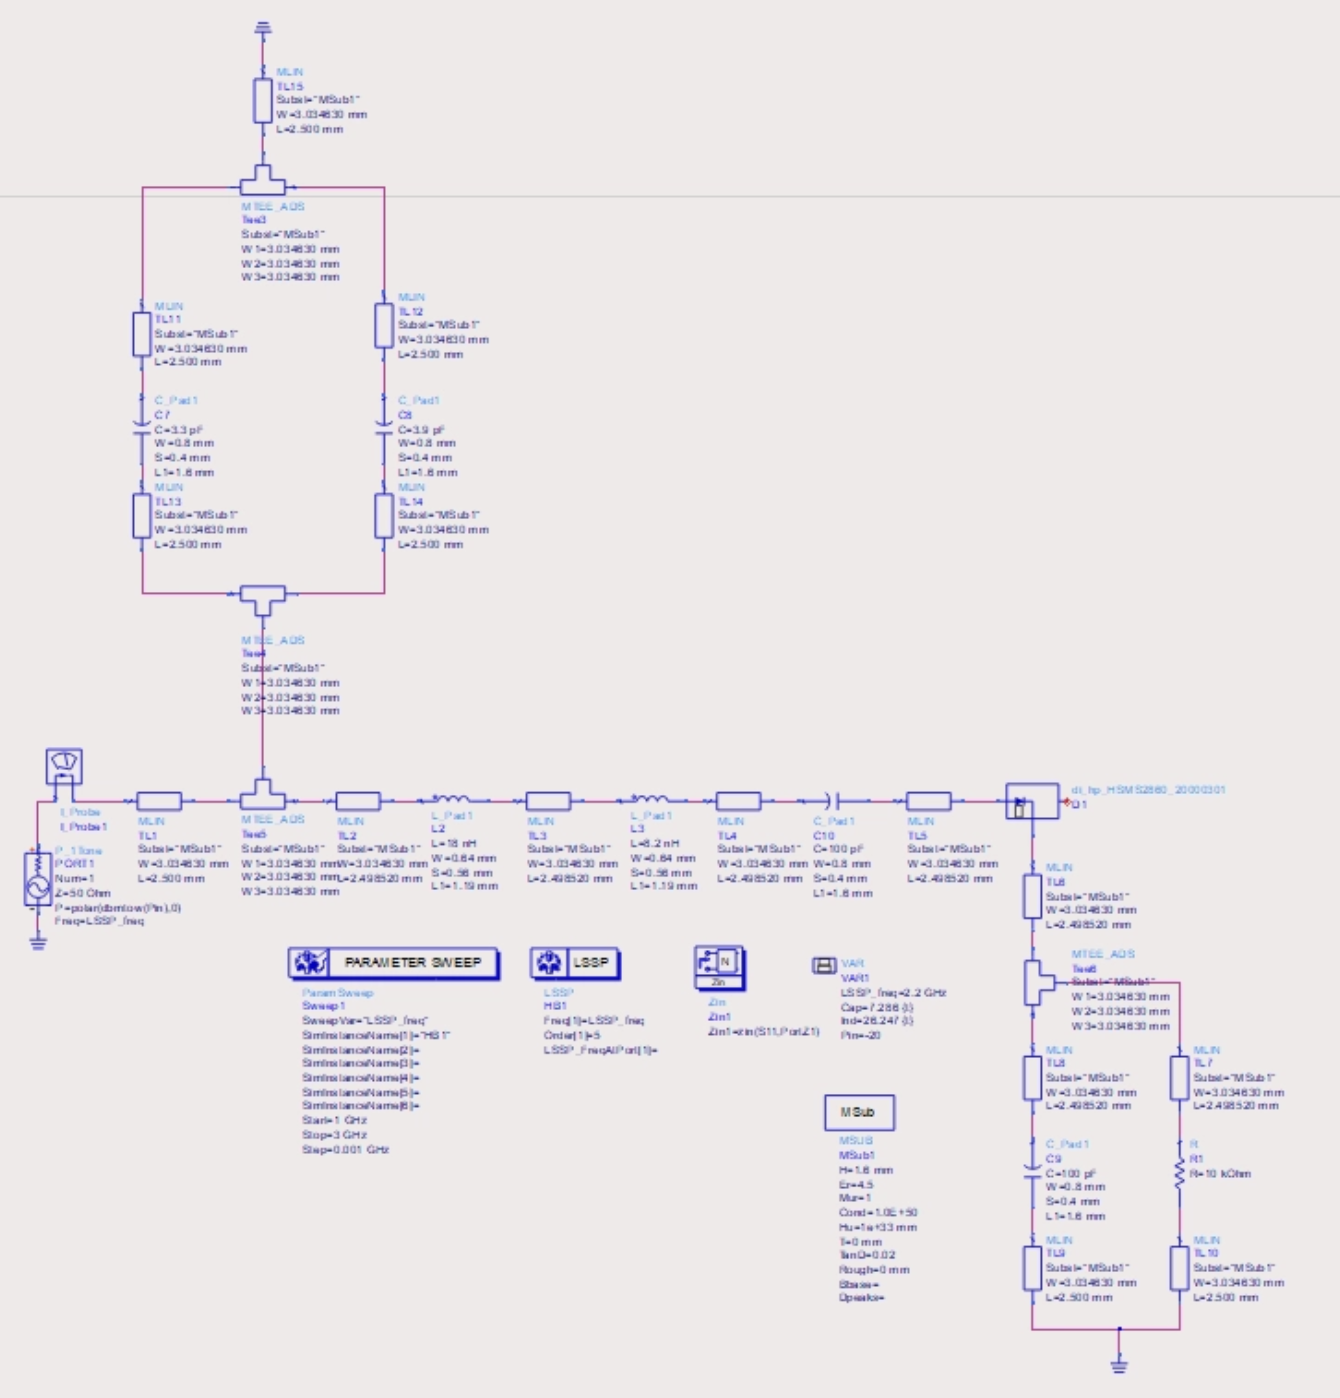
\includegraphics[width=\linewidth]{images/schema_1d_lc_ms.png}
    \caption{ADS simulation of the one-diode series rectifier, lumped-circuit and microstrip lines matching circuit.}
    \label{fig:schema_1d_lc_ms}
\end{figure}

% ------------------------------------------------------------
\subsection{Effect of microstrip parasitics on resonance frequency}
\label{subsec:mlin_parasitics}
% ------------------------------------------------------------

When the microstrip lines are introduced into the simulation while keeping
the original lumped component values unchanged, the $S_{11}$ resonance shifts from
\SI{2.2}{\giga\hertz} to approximately \SI{1.8}{\giga\hertz}
(Figure~\ref{fig:schema_1d_lc_ms}).
The degradation is caused by the additional inductance and capacitance
created by the microstrip lines, which effectively increase the total
reactive energy stored in the network.
A re-tuning of the matching circuit is therefore required to restore the
resonance at the target frequency.

\begin{figure}[H]
    \centering
    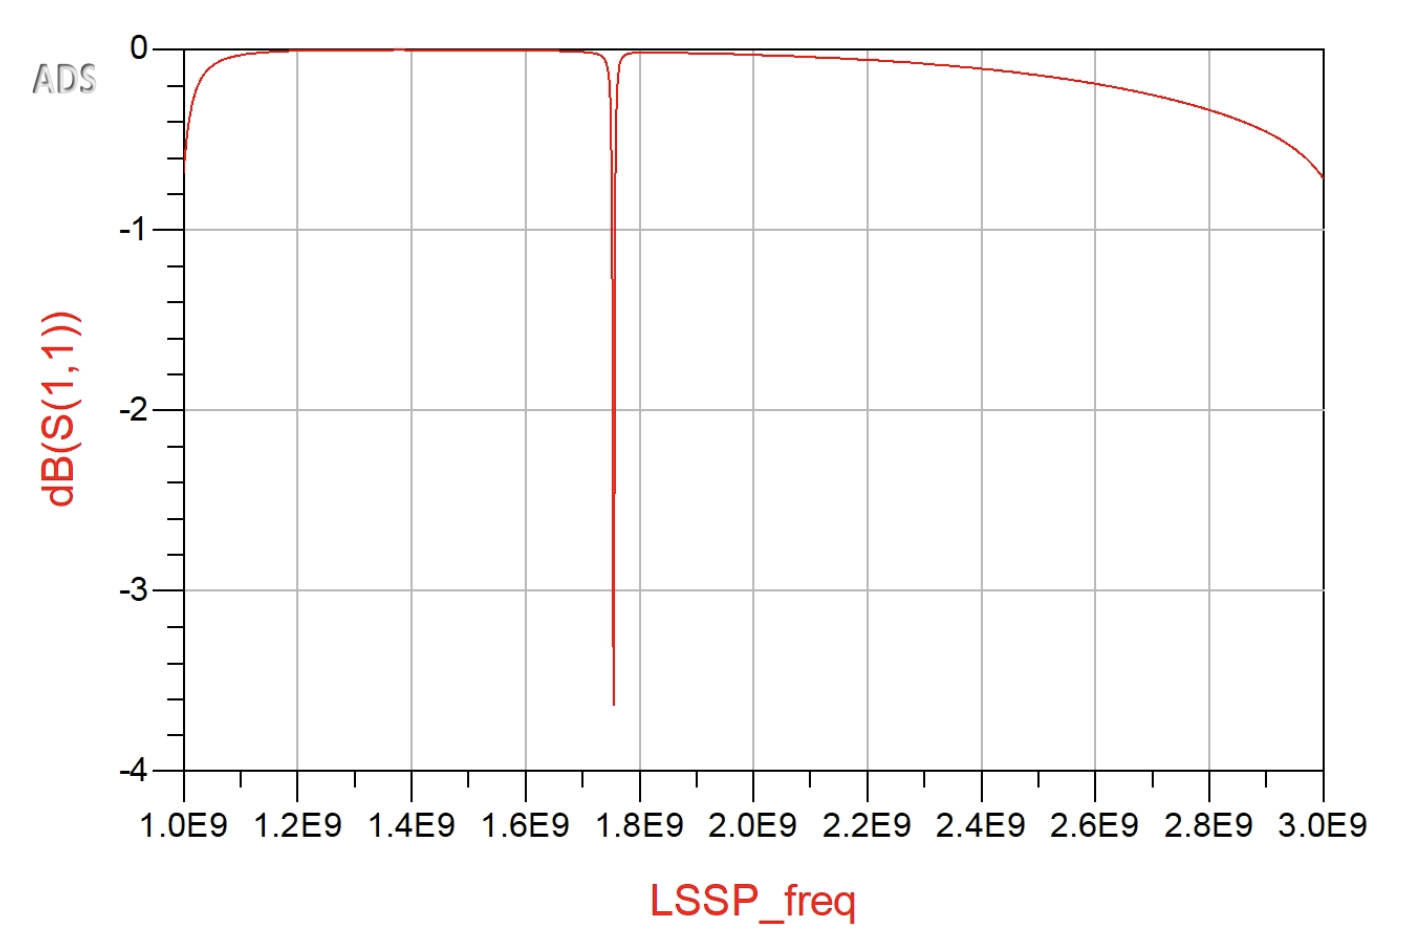
\includegraphics[width=\linewidth]{images/result_1d_S11_decale.png}
    \caption{$S_{11}$ of the lumped matching circuit with microstrip
             lines, before re-tuning.}
    \label{fig:result_1d_S11_decale}
\end{figure}

After re-tuning microstip lengths (L), capacitors (Cap) and inductors (Ind) values, we obtained these values and results : 

\begin{figure}[H]
    \centering
    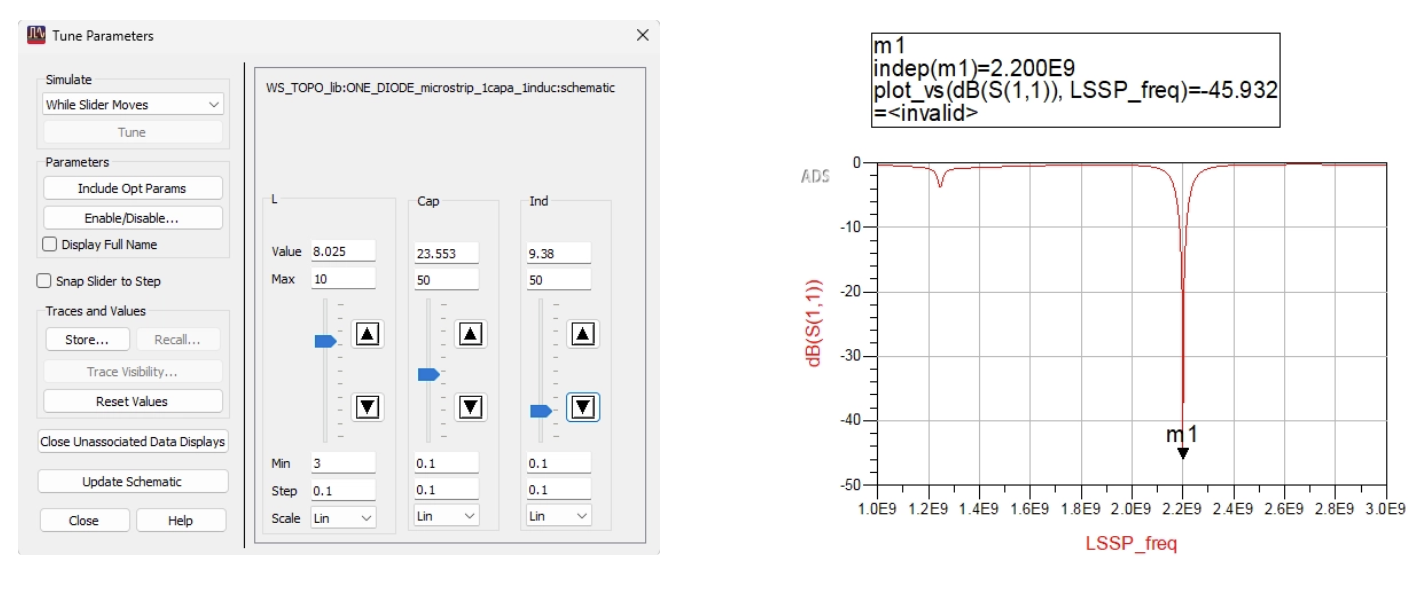
\includegraphics[width=0.75\linewidth]{images/result_1d_S11_param_lcl.png}
    \caption{$S_{11}$ of the lumped matching circuit with microstrip
            lines, after re-tuning \& parameters values.}
    \label{fig:result_1d_S11_param_lcl}
\end{figure}

By tuning our different parameters, we found right values : 
\begin{equation}
    L = \SI{8.025}{\milli\meter}, \quad
    C = \SI{23.553}{\pico\farad}, \quad
    L_\mathrm{ind} = \SI{9.38}{\nano\henry}.
\end{equation}

With those, we obtain a $S_{11}$ way below $-10$\,dB at our frequency of $2.2\,\mathrm{GHz}$ which is following specifications. 

% ------------------------------------------------------------
\subsection{Simplified 1C-1L topology with re-tuning}
\label{subsec:simplified_1c1l}
% ------------------------------------------------------------

To reduce design complexity and component count, the two-stage LC circuit is
simplified to a single capacitor and a single inductor. Here is the new schematic : 

\begin{figure}[H]
    \centering
    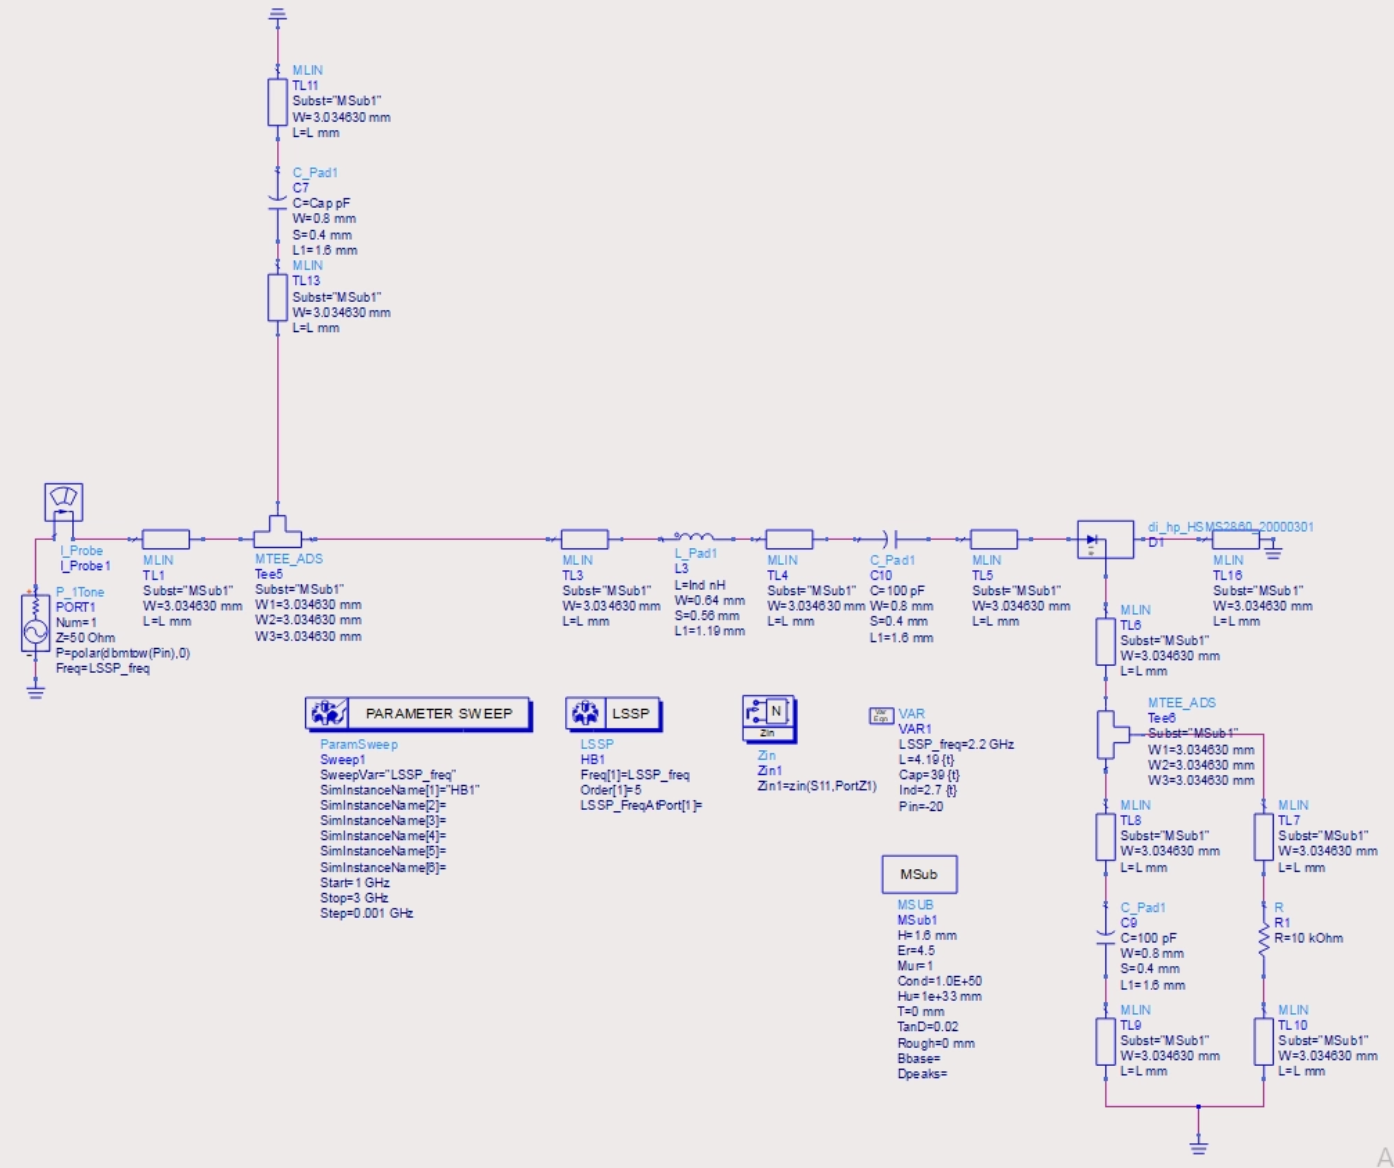
\includegraphics[width=\linewidth]{images/schema_1d_lc_ms_simple.png}
    \caption{ADS simulation of the one-diode series rectifier, lumped-circuit and microstrip lines matching circuit simplified.}
    \label{fig:schema_1d_lc_ms_simple}
\end{figure}

A parameter sweep in ADS over the line length $L$, the capacitance
$\mathrm{Cap}$, and the inductance $\mathrm{Ind}$ determined the following values:
%
\begin{equation}
    L = \SI{4.19}{\milli\meter}, \quad
    C = \SI{39}{\pico\farad}, \quad
    L_\mathrm{ind} = \SI{2.7}{\nano\henry}.
    \label{eq:opt_1c1l}
\end{equation}
%
With these values, the $S_{11}$ at \SI{2.2}{\giga\hertz} achieves:
%
\begin{align}
    S_{11} &= \SI{-31.37}{\deci\bel}
        \quad (\text{marker m1}), \\
    S_{11}&= \SI{-15.41}{\deci\bel}
        \quad (\text{marker m2}).
\end{align}
%
The results are shown in Figure~\ref{fig:s11_1c1l_retuned} :
\begin{figure}[H]
    \centering
    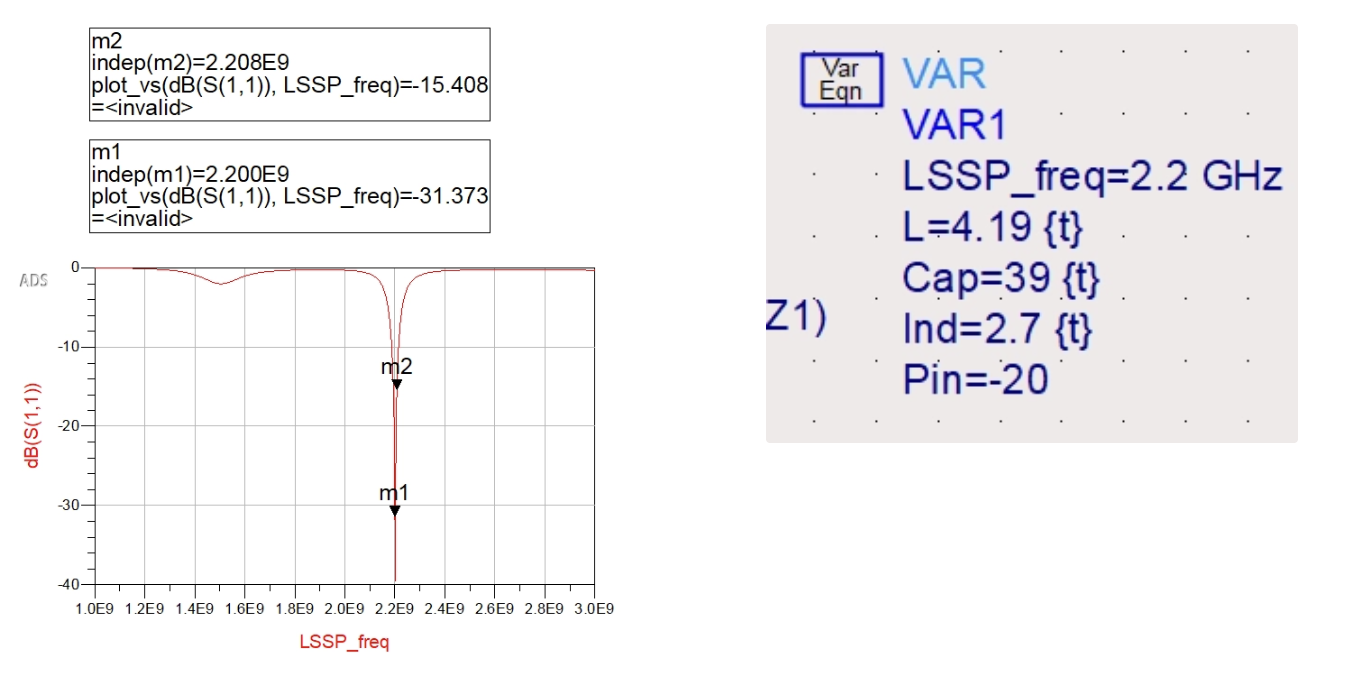
\includegraphics[width=\linewidth]{images/s11_1c1l_retuned.png}
    \caption{$S_{11}$ of the simplified 1C--1L matching circuit with
             microstrip segments, after parameter sweep re-tuning.}
    \label{fig:s11_1c1l_retuned}
\end{figure}

The specification $S_{11} < \SI{-10}{\deci\bel}$ is satisfied at \SI{2.2}{\giga\hertz},
confirming that the simplified topology is well adapted after re-tuning.

% ------------------------------------------------------------
\subsection{Fully distributed microstrip implementation}
\label{subsec:full_ms}
% ------------------------------------------------------------

For the final step, the capacitor and inductor are replaced by
microstrip lines acting as inductor and capacitor elements.
This topology eliminates the dependency on SMD components.

Here is the global schematic of this implementation : 
\begin{figure}[H]
    \centering
    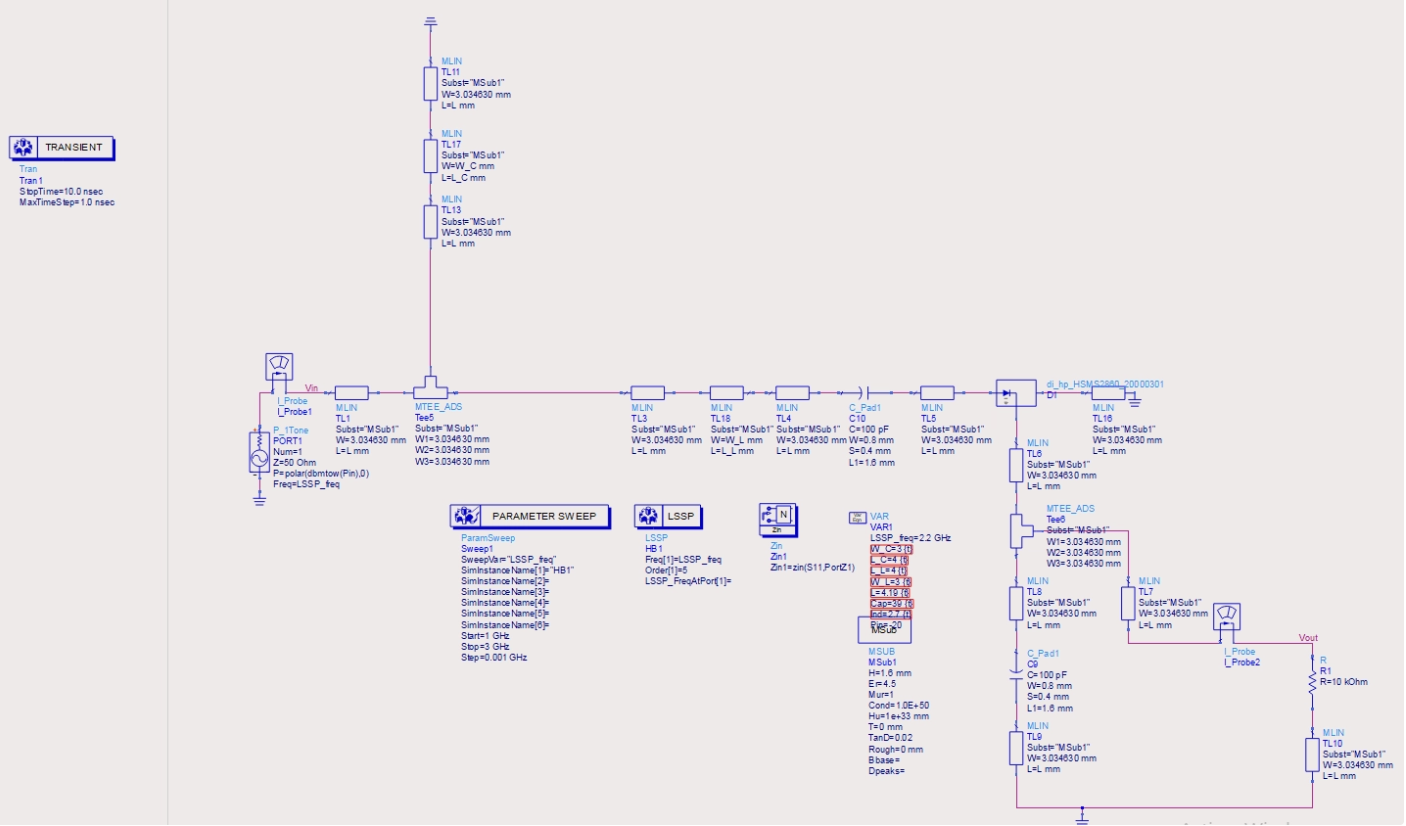
\includegraphics[width=\linewidth]{images/schema_1d_onlymc.png}
    \caption{ADS simulation of the one-diode series rectifier with only microstrip lines matching circuit.}
    \label{fig:schema_1d_onlymc}
\end{figure}

For this new implementation, new tuning have been also done for sure. Here is the result and correct parameters values : 

\begin{figure}[H]
    \centering
    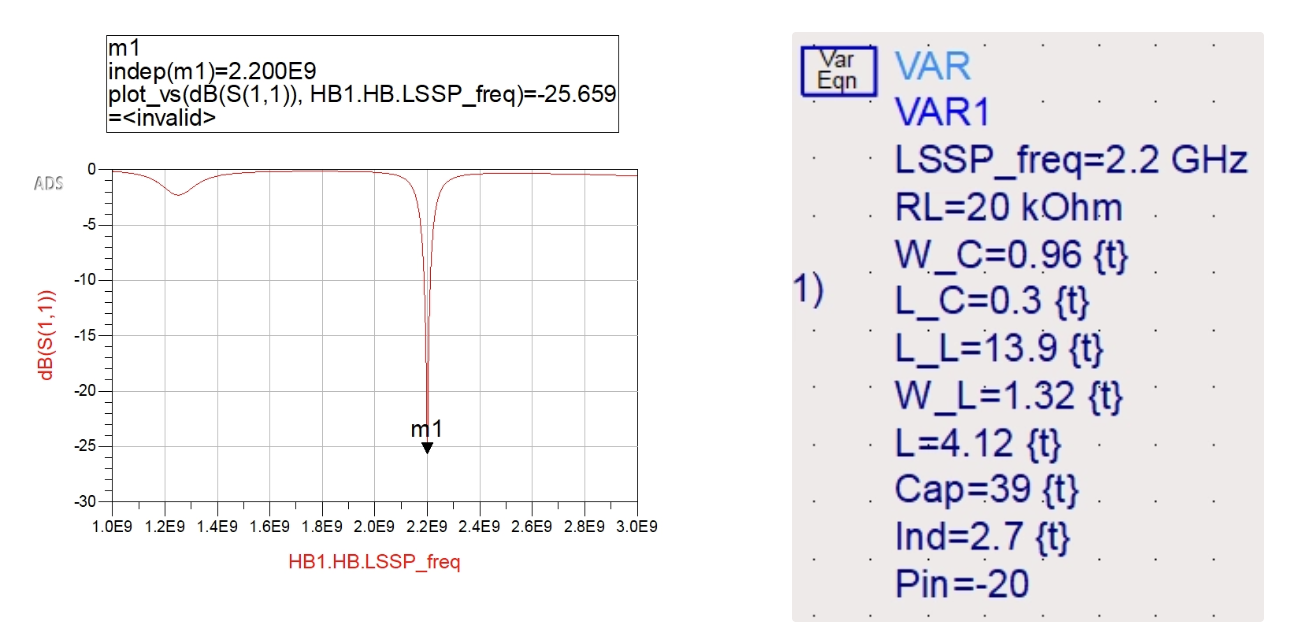
\includegraphics[width=\linewidth]{images/result_1d_onlymc.png}
    \caption{$S_{11}$ of the only microstrip lines matching circuit, after parameter sweep re-tuning.}
    \label{fig:result_1d_onlymc}
\end{figure}

The full set of tuning parameters and their optimal values after the ADS
Tune optimization are listed in Table~\ref{tab:microstrip_only_tune}.

\begin{table}[H]
    \centering
    \caption{Optimized parameter values for the full microstrip
             matching circuit (one-diode topology, \SI{2.2}{\giga\hertz}).}
    \label{tab:microstrip_only_tune}
    \begin{tabular}{lll}
        \toprule
        Parameter & Physical meaning & Optimized value \\
        \midrule
        $W_C$ & Width of capacitive stub      & \SI{0.96}{\milli\meter} \\
        $L_C$ & Length of capacitive stub     & \SI{0.3}{\milli\meter} \\
        $L_L$ & Length of inductive stub      & \SI{13.9}{\milli\meter} \\
        $W_L$ & Width of inductive stub       & \SI{1.32}{\milli\meter} \\
        $L$   & Main line segment length      & \SI{4.12}{\milli\meter} \\
        Cap   & Residual lumped capacitance   & \SI{39}{\pico\farad} \\
        Ind   & Residual lumped inductance    & \SI{2.7}{\nano\henry} \\
        \bottomrule
    \end{tabular}
\end{table}

With this fully distributed configuration, the $S_{11}$ reaches
\textbf{\SI{-25.66}{\deci\bel}} at \SI{2.2}{\giga\hertz}
(Figure~\ref{fig:result_1d_onlymc}), representing the best matching
performance achieved in this study.
The very deep and narrow resonance maximizes power transfer at our frequency at the cost of a
reduced matching bandwidth.

% ------------------------------------------------------------
\subsection{Rectifier Performance and Topology Comparison}
\label{subsec:performance_comparison}
% ------------------------------------------------------------

In this final stage, the full behavior of the one-diode topology is evaluated. We compare the ideal lumped LC matching circuit (designed in Task~3.1) with the physical microstrip circuit (designed in Task~3.2) across two main criteria: impedance matching ($S_{11}$) and RF-to-DC power conversion efficiency ($\eta$).

\subsubsection{Impedance Matching ($S_{11}$) Comparison}

Figure~\ref{fig:s11_comparison_t32} overlays the $S_{11}$ curves for the two configurations:
%
\begin{itemize}
    \item \textbf{Lumped LC circuit}: ideal SMD components, without modeling of the PCB traces;
    \item \textbf{Microstrip circuit}: capacitor and inductor replaced by physical \texttt{MLIN} blocks.
\end{itemize}

\begin{figure}[H]
    \centering
    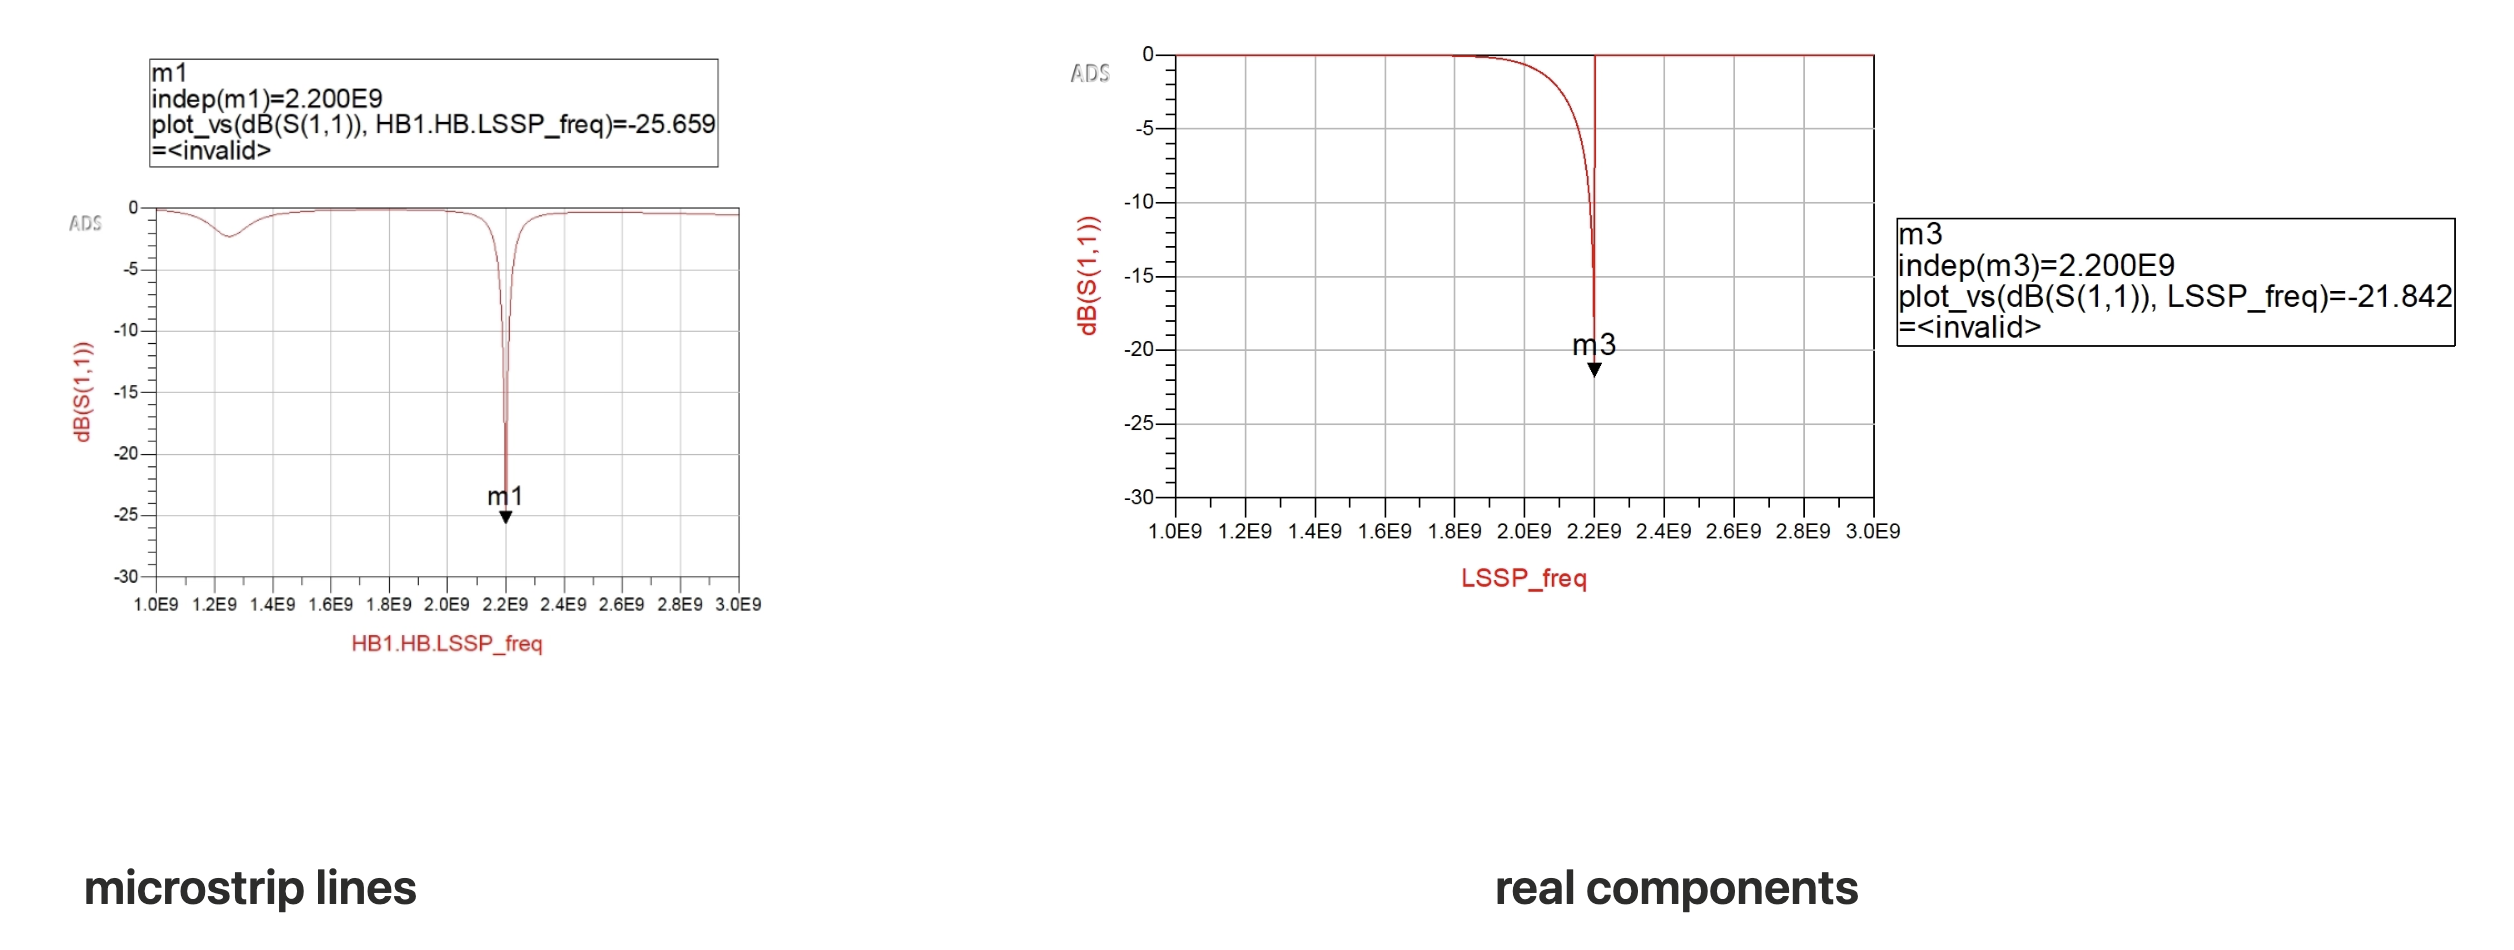
\includegraphics[width=0.75\linewidth]{images/s11_comparison_t32.png}
    \caption{Comparison of $S_{11}$ between the lumped LC matching circuit (Task~3.1) and the microstrip circuit (Task~3.2). $R_L = \SI{20}{\kilo\ohm}$, $P_\mathrm{in} = -20$\,dBm.}
    \label{fig:s11_comparison_t32}
\end{figure}

\paragraph{Impedance Matching Analysis}
Both circuits achieve to reach the right impedance matching at \SI{2.2}{\giga\hertz} ($S_{11} < \SI{-15}{\deci\bel}$), but their behaviors are quite different. The microstrip topology achieves a deeper $S_{11}$ dip, since the line dimensions allow continuous tuning, unlike the discrete values of L\&C components.
\subsubsection{Power Conversion Efficiency (\texorpdfstring{$\eta$}{eta}) and DC Output}

The RF-to-DC power conversion efficiency (PCE) is defined as the ratio of the rectified DC power delivered to the load over the incident RF power:
%
\begin{equation}
    \eta = \frac{P_\mathrm{DC}}{P_\mathrm{RF}}
         = \frac{V_\mathrm{out} \cdot I_\mathrm{out}}{V_\mathrm{in} \cdot I_\mathrm{in}}
         \times 100\,\%.
    \label{eq:pce}
\end{equation}

To accurately evaluate the performance of our system, a Large-Signal Harmonic Balance (HB) simulation was performed. The load resistance was adjusted to $R_L = \SI{20}{\kilo\ohm}$ to precisely model the equivalent input resistance of the chosen STTS22H sensor.

\paragraph{Performance of the Lumped LC Matching Circuit}
First, we simulated the topology using ideal SMD components for the matching network. Figure~\ref{fig:perf_lc_6graphs} presents the full set of results (Efficiency and Output Voltage as functions of both Input Power and Load Resistance).

\begin{figure}[H]
    \centering
    %\includegraphics[width=\linewidth]{images/perf_lc.png} % <-- Mets ici ta capture des 6 graphiques de la page 32
    \caption{Performance dashboard (Efficiency $\eta$ and $V_\mathrm{out}$) for the 1-Diode topology with Lumped LC matching ($f = \SI{2.2}{\giga\hertz}$, $R_L = \SI{20}{\kilo\ohm}$).}
    \label{fig:perf_lc_6graphs}
\end{figure}

At our maximum targeted input power ($P_\mathrm{in} = \SI{10}{\dBm}$), the efficiency reaches approximately \textbf{6.69\%}.

\paragraph{ Performance of the Full Microstrip Circuit}
Next, we evaluated the final physical implementation where the matching network relies solely on microstrip lines. The results are shown in Figure~\ref{fig:perf_ms_6graphs}.

\begin{figure}[H]
    \centering
    %\includegraphics[width=\linewidth]{images/perf_ms.png} % <-- Mets ici ta capture des 6 graphiques de la page 33
    \caption{Performance dashboard (Efficiency $\eta$ and $V_\mathrm{out}$) for the 1-Diode topology with fully distributed Microstrip matching ($f = \SI{2.2}{\giga\hertz}$, $R_L = \SI{20}{\kilo\ohm}$).}
    \label{fig:perf_ms_6graphs}
\end{figure}

With the microstrip matching network, the efficiency at $P_\mathrm{in} = \SI{10}{\dBm}$ improves drastically, reaching \textbf{17.15\%}. 

\paragraph{Efficiency Analysis}
This significant improvement (from 6.69\% to 17.15\%) can be explained by the physical nature of the matching networks. Ideal lumped inductors and capacitors have inherent parasitic series resistances ($R_s$) that dissipate RF energy as heat. By replacing them with fully distributed microstrip lines on a high-quality RF substrate (Rogers 4350B), we reduce these insertion losses, leading to a higher quality factor (Q) and better energy transfer to the diode.

\subsubsection{Adequacy for powering the STTS22H sensor}

The ultimate goal of this rectifier is to power an STTS22H temperature sensor. According to its datasheet, the sensor requires a supply voltage between \SI{1.5}{\volt} and \SI{3.6}{\volt}, and consumes a maximum active current of \SI{120}{\micro\ampere}. 

The absolute minimum DC power required is:
%
\begin{equation}
    P_\mathrm{DC,min}
    = V_\mathrm{DD,min} \times I_\mathrm{DD,max}
    = \SI{1.5}{\volt} \times \SI{120}{\micro\ampere}
    = \SI{180}{\micro\watt}.
\end{equation}

Using our final microstrip implementation at an input power of $P_\mathrm{in} = \SI{10}{\dBm}$ (which equals \SI{10}{\milli\watt}), the measured efficiency is $\eta = 17.15\%$. 
The delivered DC power is therefore:
\begin{equation}
    P_\mathrm{DC,delivered} = \SI{10}{\milli\watt} \times 0.1715 = \SI{1.715}{\milli\watt} = \SI{1715}{\micro\watt}.
\end{equation}

\paragraph{Conclusion}
The delivered power (\SI{1715}{\micro\watt}) is nearly ten times higher than the strict minimum required (\SI{180}{\micro\watt}). Furthermore, the Harmonic Balance simulation (Figure~\ref{fig:perf_ms_6graphs}) shows that at $P_\mathrm{in} = \SI{10}{\dBm}$, the output voltage $V_\mathrm{out}$ reaches approximately \SI{2.5}{\volt} to \SI{3.0}{\volt}, which sits perfectly within the sensor's safe operating range (\SIrange{1.5}{3.6}{\volt}). 

We can confidently conclude that the one-diode microstrip topology is fully capable of powering the STTS22H sensor under these RF conditions.

% ==========================================
% BIBLIOGRAPHIE
% ==========================================
\bibliographystyle{IEEEtran}
% \bibliography{biblio}

\end{document}